\documentclass[12pt]{article}

\usepackage{sbc-template}

\usepackage{graphicx,url}

\usepackage[brazil]{babel}   
%\usepackage[latin1]{inputenc}  
\usepackage[utf8]{inputenc}  
% UTF-8 encoding is recommended by ShareLaTex

     
\sloppy

\title{Teoria dos Grafos - Trabalho Final\\ Projeto 3}

\author{Adriano Zanella Junior\inst{1}, Marlon Henry Schweigert\inst{2}}


\address{Centro de Ciências Tecnológicas --\\ Universidade do Estado de Santa Catarina (UDESC) -- DCC
}

\begin{document} 

\maketitle
     
\begin{resumo} 
    Este artigo apresenta a problemática do projeto que será solucionado pela equipe, assim como sua interpretação, sua modelagem e a solução do problema dado pelo projeto.
\end{resumo}


\section{Contexto do Problema}
    
O projeto 3 supõe que uma pessoa, que chamaremos de chefe, queira encontrar o segundo menor caminho em uma cidade de um ponto a outro, tendo em vista que os caminhos mínimos estejam sendo usado por muitas pessoas, causando congestionamento neles. Assim, o segundo menor caminho deve ser mais rápido mesmo que mais longo. O problema ainda cita que pode não haver uma solução. 

O segundo menor caminho não deve possuir nenhuma rua em comum com o menor caminho. Por exemplo, na imagem abaixo existem dois caminhos mínimos de S a D de custo 8 (em azul). O caminho  com o segundo valor minimo de custo 9 (em vermelho) possui ruas em comum com o caminho mínimo, estas ruas devem estar congestionadas e não são de interesse do chefe. O caminho de segundo menor custo e sem ruas comuns aos caminhos de menor custo possui custo 11 (em verde).

\begin{figure}[ht]
    \centering
    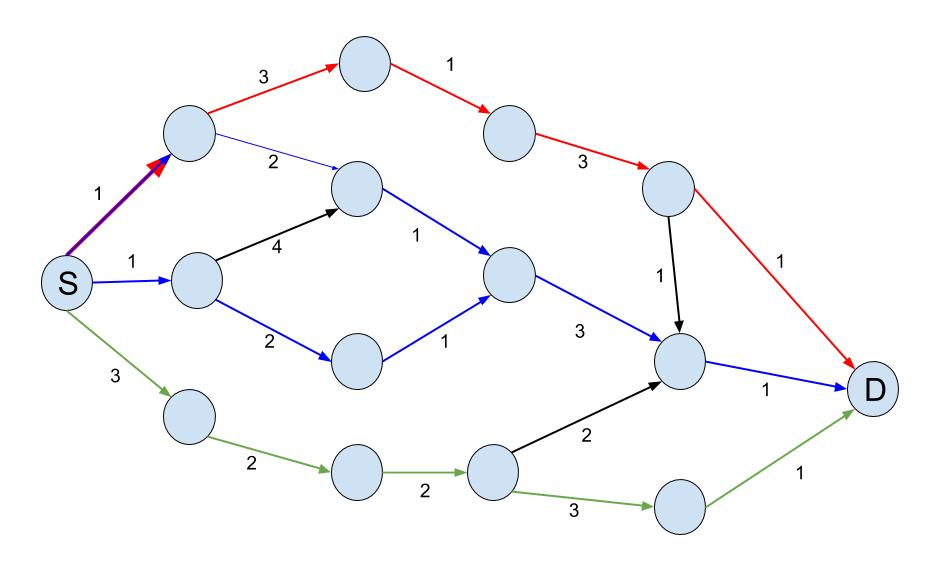
\includegraphics[width=.85\textwidth]{TEGexempleColor.jpg}
    \caption{Quase menor caminho.}
    \label{fig. 1:}
\end{figure}


\section{Interpretação} 

Como pretende-se ir de um ponto a outro, será utilizado um grafo de fluxo, com uma origem e um sumidouro. O problema pede o quase caminho de menor custo, e para isso será necessário dos caminhos de menor custo.

O problema neste caso é encontrar o caminho de segundo menor custo que não possua  arestas em comum com o caminho de menor custo. Para isso deveremos uma vez que tenhamos os caminhos de menor custo, ignorar as ruas (arestas) que estes caminhos utilizem. 

Ignorando essas ruas (arestas) devemos ser capazes de encontrar pelo menos um caminho completamente distinto dos caminhos de menor custo, ou nenhum caminho, o que representa que não existe um caminho que passe por pelo menos uma rua dos caminhos de  menor custo.


\section{Modelagem do Problema}

O problema nos oferece o modelo de entrada como primeiramente dois inteiros sendo o numero de vértices e o numero de arestas consecutivamente. Seguindo de dois inteiros, o vértice de origem e de destino. A seguir uma lista das arestas contendo a origem desta, o peso, e o destino.

Para o grafo utilizamos uma matriz de adjacência, por ser mais simples de implementar e mais fácil de mover pelo grafo. O grafo criado é um grafo direcionado, uma vez que o problema cita que são ruas de via única.

Para encontrar o caminho de menor custo e o caminho de segundo menor custo foi utilizado o algorítimo de Dijkstra, que busca o caminho de menor custo de um vértice a outro, assim marcaremos os caminhos de menor custo para remoção posterior.


\section{Solução do Problema}

Para resolver o problema proposto, foi criado um algorítimo que lê as entradas para montar o grafo segundo as especificações do projeto e possui uma saída contendo o custo do quase menor caminho ou -1 caso não exista um quase menor caminho válido.
 
Com as entradas é criado um grafo de adjacência em que é aplicado o algorítimo de Dijkstra da origem ao sumidouro, marcando os vértices pertencentes aos caminhos de menor custo. Após o algorítimo de Dijkstra realizar sua função, é realizado uma função para remover as arestas marcadas, assim retiramos os caminhos de menor custo do grafo, para logo após realizar o Dijkstra novamente. Desta vez obteremos o quase caminho de menor custo, sem nenhuma das arestas em comum com os caminhos de menor custo, ou não obteremos nenhum caminho, caso a fonte se torne inalcançável. Neste caso retornamos um -1. 

Caso exista o quase caminho de menor custo, retornaremos o seu custo.


\section{Conclusão}

Com o algorítimo finalizado, o chefe terá seu tempo entre dois pontos reduzido, mesmo tendo de percorrer um caminho mais longo, ou terá de utilizar as vias mais concorridas caso não exista um quase caminho de menor custo.


\end{document}
